\documentclass[../integrointiopas.tex]{subfiles}
\graphicspath{{\subfix{../kuvat/}}}

\begin{document}
	Yhden muuttujan tapauksessa mielivaltaisen funktion $f(x)$ integraalifunktion $F(x)$ määrittelee ehto:
	
	\begin{equation}
		F'(x) = f(x)
	\end{equation} 
	
	Tällöin funktion $f$ määräämätön integraali on integroimisvakiota $C$ vaille $f$:n integraalifunktio $F$:
	
	\begin{equation}
		\int f(x)\odif{x} = F(x) + C
	\end{equation} 
	
	Yhden muuttujan funktioiden määrättyjen integraalien määrittäminen perustuu myös integraalifunktioon:
	
	\begin{equation}
		\int_{a}^{b}f(x)\odif{x} = F(x)\bigg|_a^{b} = F(b) - F(a)
	\end{equation}
	
	Yhtälö (4.3) kertoo, että funktion $f$ integraalin määrittämiseksi välillä $x\in[a, b]$ riittää määrittää $f$:n integraalifunktion $F$ arvojen erotus välin päätepisteissä $a$ ja $b$. Havaitaan, että oli sitten kyseessä määräämätön tai määrätty integraali, on integraalifunktion $F$ määrittäminen välttämätöntä integroinnin suorittamiseksi. Integrointimenetelmät ovatkin tapoja määrittää integraalifunktio $F$, kun lähdetään liikkeelle integroitavasta funktiosta, eli integrandista $f$. Osioissa 4.1 - 4.N käydään läpi tärkeimmät menetelmät yhden muuttujan funktioiden integroimiseksi. 
	
	\subsection{Alkeisfunktioiden integrointi}
	
	Alkeisfunktiot ovat yhden muuttujan funktioita, jotka voidaan muodostaa käyttämällä ainoastaan aritmeettisia operaatioita, funktion tai käänteisfunktion ottamista sekä funktioiden yhdistämistä. Alkeisfunktiot ovat hyvin käyttäytyviä sekä melko helposti integroituvia ja ovatkin tästä syystä oiva paikka aloittaa integrointimenetelmien harjoittelu. Alkeisfunktioihin kuuluu polynomi-, juuri-, rationaali, eksponentti- ja logaritmifunktiot sekä trigonometriset ja hyperboliset funktiot että näiden käänteisfunktiot. Osioissa 4.1.1 - 4.1.5 käydään läpi kaikkien alkeisfunktioiden integrointi.
	
	\subsubsection{Polynomi- ja juurifunktioiden integrointi}
	
	Yhden muuttujan polynomifunktio $P_n(x) = ax^n + bx^{n - 1} + \dots + px + q$, jossa $n$ on polynomin asteluku eli korkein siinä esiintyvä potenssi, on kenties alkeisfunktiotyypeistä suoraviivaisin integroida. Tämä johtuu siitä, että polynomifunktioita integroitaessa voidaan suoraan soveltaa derivaattojen laskennasta tuttua potenssifunktion derivaattaa käänteiseen suuntaan. Tiedetään, että yleiselle potenssifunktiolle $x^n$ pätee:
	
	\begin{equation}
		\odv{}{x}x^n = nx^{n - 1}
	\end{equation}
	
	Toisaalta tiedetään, että integrointi on derivoinnin käänteisoperaatio, jolloin tulee päteä:
	
	\begin{equation}
		\int nx^{n - 1}\odif{x} = x^n + C
	\end{equation}
	
	Kun nyt tarkastellaan, miten integrointi muutti funktiota havaitaan, että integrandin asteluku kasvoi yhdellä $n - 1 \to n$ ja etukerroin $n$ katosi kokonaan ikään kuin $nx^{n - 1}$ olisi jaettu $n$:llä. Koska $n$ on vain jokin kokonaislukumuuttuja, voidaan se nimetä uudelleen $n \to n + 1$, jolloin saadaan:
	
	\begin{equation}
		\int (n + 1)x^{n}\odif{x} = x^{n + 1} + C
	\end{equation}
	
	Jälleen $x$:n potenssi kasvoi yhdellä ja etukerroin jakautui pois, kun integrandi jaettiin $n + 1$:llä. Jos nyt sovelletaan samaa ajatteluketjua alkuperäiselle potenssifunktiolle $x^n$, saadaan eksponenttia kasvattamalla ja $n + 1$:llä jakamalla yleinen tulos potenssifunktioiden integroinnille:
	
	\begin{equation}
		\boxed{\int x^n\odif{x} = \frac{1}{n + 1}x^{n + 1} + C} 
	\end{equation}
	
	Koska polynomit ovat vain summa eriasteisia $x$:n potensseja ja integrointi voidaan suorittaa summan termeille erikseen ottamalla mahdolliset vakiotermit integraalin etukertoimiksi (lineaarisuus), voidaan mielivaltaiselle polynomille $P_n(x)$ kirjoittaa:
	
	\begin{align}
		\int P_n(x)\odif{x} &= \int (ax^n + bx^{n - 1} + \dots + px + q)\odif{x} \\
		&= a\int x^n\odif{x} + b\int x^{n - 1}\odif{x} + \dots + p\int x\odif{x} + q\int\odif{x}
	\end{align}
	
	Soveltamalla tulosta (4.7) saadaan polyomeille yleisesti pätevä tulos:
	
	\begin{equation}
		\boxed{\int P_n(x)\odif{x} = \frac{a}{n + 1}x^{n + 1} + \frac{b}{n}x^n + \dots + \frac{p}{2}x^2 + qx + C}
	\end{equation}
	
	Entä jos potenssiin korotetaan yksittäisen muuttujan sijasta jokin polynomi? Tarkastellaan esimerkiksi funktion $f(x) = (ax + b)^2$ integraalia:
	
	\begin{equation}
		\int(ax + b)^2\odif{x}
	\end{equation}
	
	Integraali voidaan ratkaista samalla tavalla kuin aiemmin, kunhan vain sulut ensin avataan ja saatetaan integrandi polynomin $P_n(x)$ kaltaiseen muotoon:
	
	\begin{align}
		\int(ax + b)^2\odif{x} &= \int(a^2x^2 + 2abx + b^2)\odif{x} \\
		&= a^2\int x^2\odif{x} + 2ab\int x\odif{x} + b^2\int\odif{x} \\
		&= \frac{a^2}{3}x^3 + abx^2 + b^2x + C
	\end{align}
	
	Vastaavanlaista argumentointia voidaan käyttää määrittämään minkä tahansa polynomifunktion integraali, jossa esiintyy useamman termin kokonaislukupotensseja.
	
	Tarkastellaan seuraavaksi juuifunkitoita. Ne saadaan yleistämällä potenssifunktiot murtopotensseihin ja ne käyttäytyvätkin hyvin samanlaisella tavalla potenssifunktioihin verrattuna integroitaessa. Täysin mielivaltaiselle murtopotenssifunktiolle $x^{\frac{m}{n}}$ pätee sama potenssin integrointisääntö kuin aiemmin:
	
	\begin{equation}
		\boxed{\int x^{\frac{m}{n}}\odif{x} = \frac{n}{m}x^{\frac{m}{n} + 1} + C}
	\end{equation}
	
	Murtopotenssien erikoistapaus ovat juuret, jotka saadaan, kun $m = 1$. Juurifunktioiden integraaleille voidaankin siis kirjoittaa yleisesti:
	
	\begin{equation}
		\boxed{\int \sqrt[n]{x}\odif{x} = \int x^{\frac{1}{n}}\odif{x} = nx^{\frac{1}{n} + 1} + C = n\sqrt[n]{x^{n+1}} + C}
	\end{equation}
	
	Entä jos juuren alla on useampi termi? Koska juuria ei voi avata samalla tavalla kuin polynomien potensseja, jäävät tämänkaltaiset integraalit vielä tässä vaiheessa ratkaisemattomiksi, mutta palaamme tämänkaltaisiin integraaleihin osiossa 4.2.
	
	
	
	\subsubsection{Rationaalifunktioitden integrointi}
	
	Rationaalifunktiot $r(x)$ ovat funktioita, jotka voidaan kirjoittaa muodossa
	
	\begin{equation}
		r(x) = \frac{p(x)}{q(x)}
	\end{equation}
	
	ja jossa $p(x)$ ja $q(x)$ ovat mielivaltaisia polynomifunktioita. Yleisessä tapauksessa rationaalifunktioiden integrointi perustuu siihen, että osamäärä $p(x)/q(x)$ ilmaistaan usean yksinkertaisemman osamäärän summana tekemällä osamäärälle nk. osamurtokehitelmä. Kun osamäärä on ilmaistu yksinkertaisten osien summana, voidaan integrointi suorittaa kullekin termille erikseen lopputuloksen saamiseksi. 
	
	Ennen osamurtokehitelmiin siirtymistä tarkastellaan kuitenkin yhtä yksinkertaista erikoistapausta rationaalifunktiosta, joka kuuluu myös edellisessä osiossa tarkasteltuihin potenssifunktioihin mutta jonka integraalia emme itseasiassa vielä osaa määrittää: käänteislukufunktio $\frac{1}{x} = x^{-1}$. Käänteislukufunktio muistuttaa ulkoisilta ominaisuuksiltaan funktiota, jonka integraali voitaisiin yksinkertaisesti määrittää soveltamalla kaavaa (4.7). Kaavassa piilee kuitenkin ongelma, joka tulee nimenomaan esille käänteislukufunktion kanssa: kun integroidaan potenssifunktiota, kasvaa muuttujan eksponentti yhdellä, jolloin käänteislukufunktion eksponentiksi tulisi $-1 + 1 = 0$. Tämä on jo hieman huolestuttavaa, sillä funktio $x^0$ on vain vakiofunktio $1$, eikä vakiofunktion derivaatta ole käänteislukufunktio, vaan nollafunktio. Suurempi ongelma tulee kuitenkin vastaan kun jaetaan uudella eksponentilla, eli nollalla. Käänteislukufunktion integraali on siis $\frac{1}{0}$! Tulos on tottakai virheellinen, mutta herättää kysymyksen: miten integraali tulisi määrittää? Tässä vaiheessa derivaattoja tunteva henkilö saattaa muistaa, että luonnollisen logaritmin $\ln(x)$ (joskus myös $\log(x)$) derivaatta on käänteislukufunktio $\frac{1}{x}$, kun $x > 0$. Toisin sanoen pätee:
	
	\begin{equation}
		\odv{}{x}\ln(x) = \frac{1}{x}, \ \ x > 0
	\end{equation}

	Vaatimus $x > 0$ on tärkeä, sillä luonnollinen logaritmi on määritelty reaaliluvuille vain positiivisilla argumenteilla, kun taas käänteisluvun voi ottaa mistä tahansa nollasta poikkeavasta luvusta jolloin on valittava määrittelyehdoista rajoittavampi koko yhtälön määrittelyehdoksi. Kun nyt muistetaan yhtälö (4.1), joka määrittelee integraalifunktion käsitteen, voidaan tehdä seuraavat samaistukset: $F'(x) = \odv{}{x}\ln(x)$ ja $f(x) = \frac{1}{x}$. Tällöin yhtälön (4.2) nojalla pätee:
	
	\begin{equation}
		\int \frac{1}{x}\odif{x} = \ln(x) + C, \ \ x > 0
	\end{equation}

	Käänteislukufunktion integraalifunktio on siis luonnollinen logaritmi! Tulos (4.19) ei kuitenkaan ole integraalifunktion lopullinen muoto, sillä se sisältää kömpelön vaatimuksen $x$:n positiivisuudesta, jolloin sitä ei voida käyttää, jos esim. määritetään funktion $\frac{1}{x}$ määrätty integraali välillä $[-2, -1]$. Vaatimuksesta päästään eroon ottamalla logaritmin argumentista itseisarvo, sillä funktion $\frac{1}{x}$ kuvaaja on etumerkkiä vaille symmetrinen y-akselin suhteen jolloin pinta-alaa kertyy samalla tahdilla y-akselin molemmilla puolilla ja negatiivisen välin yli integroiminen tuottaa saman tuloksen kuin vastaavan positiivisen välin yli integroiminen. Käänteislukufunktion integraalille saadaan siis lopulta relaatio:
	
	\begin{equation}
		\boxed{\int \frac{1}{x}\odif{x} = \ln|x| + C}
	\end{equation}

	Tulos (4.20) antaa mielikuvan siitä, että osamäärien integroiminen ja luonnollinen logaritmifunktio ovat jollakin tavalla linkittyneet toisiinsa. Tämä on oikea intuitio, ja tulemme törmäämään luonnolliseen logaritmiin vielä paljon, kun lähdemme seuraavaksi tarkastelemaan monimutkaisempien rationaalifunktioiden integrointia. \\
	
	\noindent\textbf{Osamurtokehitelmät} \\
	
	Kuten osion $4.1.2$ alussa todettiin, perustuu rationaalifunktioiden $r(x) = \frac{p(x)}{q(x)}$ integroiminen nk. osamurtokehitelmän tekemiseen. Osamurtokehitelmässä on ideana ottaa jokin rationaalifunktio, esim.
	
	\begin{equation}
		r(x) = \frac{3x - 10}{x^2 - 7x + 12}
	\end{equation}

	ja ilmaista se nimittäjän $x^2 - 7x + 12$ nollakohtien $x = 3$ ja $x = 4$ avulla muodossa
	
	\begin{equation}
		r(x) = \frac{1}{x - 3} + \frac{2}{x - 4}
	\end{equation}

	Ylläoleva muoto on tämän jälkeen suoraviivaista integroida, kun käänteislukufunktion $\frac{1}{x}$ integraali tunnetaan. Kuinka ylläolevaan muotoon sitten päästään ja miksi sillä on mitään tekemistä nimittäjän juurien kanssa? Tarkastellaan tätä seuraavaksi.
	
	Osamurtokehitelmien tekeminen perustuu algebran peruslauseeseen, joka sanoo yksinkertaisuudessaan että $n$:nen asteen polynomilla on tasan $n$ juurta (mikäli tuplajuuret lasketaan kahdeksi, triplajuuret kolmeksi jne.) kompleksilukujen joukossa. Koska juuret ovat pisteitä, jossa polynomi menee nollaan, voidaan mikä tahansa polynomi 
	
	\begin{equation}
		s(x) = a_0x^n + a_1x^{n-1}+\dots+a_{n-1}x + a_n
	\end{equation}
	
	 ilmaista sen erään juuren $j_1$ ja polynomin $t(x)$ tulona muodossa
	 
	 \begin{equation}
	 	s(x) = (x - j_1)t(x)
	 \end{equation}
 
 	Kun lausekeeseen sijoittaa $x = j_1$, menee ensimmäinen termi $(x - j_1) = (j_1 - j_1)$ nollaan, eli $j_1$ on edelleen $s(x)$:n juuri. Kun tätä jatketaan kaikille $s(x)$:n juurille, saadaan $s(x)$ ilmaistua juurtensa $j_i$ tulona: 
 	
 	\begin{equation}
 		s(x) = a_0(x - j_1)(x - j_2)\dots(x - j_n)
 	\end{equation}
	
	Murtolukujen ominaisuuksista seuraa, että esimerkiksi murtolukujen summa $\frac{A}{a} + \frac{B}{b} + \frac{C}{c}$ voidaan ilmaista yhtenä murtolukuna
	
	\begin{equation}
		\frac{A}{a} + \frac{B}{b} + \frac{C}{c} = \frac{Abc + Bac + Cab}{abc},
	\end{equation}

	jossa murtoluvun nimittäjä on alkuperäisten murtolukujen nimittäjien tulo. Kun tulkitaan luvut $a$, $b$ ja $c$ jonkin polynomin tekijöiksi $(x - j_i)$, huomataan että soveltamalla ajattelua toiseen suuntaan voidaan jokin rationaalifunktio, jonka nimittäjä on jaettu tekijöihin $\frac{Abc + Bac + Cab}{abc}$ ilmaista summalausekkeena $\frac{A}{a} + \frac{B}{b} + \frac{C}{c}$, jossa murtolukujen nimittäjissä esiintyy alkuperäisen nimittäjän tekijät ja osoittajissa oikein valitut termit $A$, $B$ ja $C$. Osamurtokehitelmien tekeminen vastaakin juuri näiden termien $A$, $B$ ja $C$ löytämistä (korkeamman asteen tapauksessa termejä on enemmän, toisen asteen tapauksessa vain kaksi) alkuperäisen rationaalifunktion avulla. On tärkeää huomata, että missään vaiheessa ei otettu kantaa juurten $j_i$ moninkertaan. Tekijät $a$, $b$ ja $c$ voivat siis olla yleisessä tapauksessa muotoa $(x - j_i)^m$, jossa $m\in\mathbb{Z}_+$ on juuren $j_i$ moninkerta. 
	
	Nyt olemme valmiita tarkastelemaan osamurtokehitelmien tekemistä tarkemmin. Olen jakanut rationaalifunktiot kolmeen kategoriaan, joille osamurtokehitelmän tekeminen on edellistä hieman työläämpi prosessi. Kun kunkin kategorian funktioiden osamurtokehitelmien tekeminen on lukijalle tuttu, kykenee tämä suorittamaan osamurtokehitelmiä teoriassa mille tahansa rationaalifuntkiolle. (Toki todellisuudessa osamurtokehitelmän tekeminen ei aina ole paras tapa jonkin integraalin ratkaisemiseen tai vaihtoehtoisesti kehitelmän tekeminen voi olla polynomien korkean asteluvun vuoksi äärimmäisen työläs prosessi ilman tietokoneen avustusta). \\
	
	\begin{enumerate}
		\item \textbf{Nimittäjän asteluku korkeampi kuin osoittajan ja nimittäjällä vain yksinkertaisia juuria}
		
		Tarkastellaan siis muotoa
		
		\begin{equation}
			r(x) = \frac{p_n(x)}{q_m(x)}
		\end{equation}
	
		olevia rationaalifunktioita, jossa $n$ on $p$:n asteluku, $m$ on $q$:n asteluku ja $m > n$. Lisäksi $q$:n tekijöihin jako sisältää vain yksinkertaisia juuria, eli:
		
		\begin{equation}
			r(x) = \frac{p_n(x)}{(x - j_1)(x - j_2)\cdots(x - j_m)}
		\end{equation}
	
		Yhtälössä (4.28) rationaalifunktiota on supistettu siten, että $q$:n korkeimman asteen termin kerroin on 1, jolloin tekijöihin jako vastaa yhtälöä (4.25) kerrointa $a_0$ lukuunottamatta. Kirjoitetaan nyt tuloksen (4.26) kautta saadun idean perusteella rationaalifunktio termien $\frac{A_i}{x - j_i}$ summana. Oletetaan yksinkertaistuksen vuoksi, että $q$ on kolmannen asteen polynomi, jolloin sillä on kolme tekijää. (Metodi toimii vastaavalla tavalla korkeammillekin asteille, mutta tämän tekeminen yleisessä muodossa on haastavaa.):
		
		\begin{align}
			&\frac{p(x)}{(x - j_1)(x - j_2)(x - j_3)} = \frac{A_1}{x - j_1} + \frac{A_2}{x - j_2} + \frac{A_3}{x - j_3} \\
			\intertext{Tarkastellaan yhtälön oikeaa puolta. Lavennetaan termit samannimisiksi:}
			&\frac{A_1(x - j_2)(x - j_3) + A_2(x - j_1)(x - j_3) + A_3(x - j_1)(x - j_2)}{(x - j_1)(x - j_2)(x - j_3)} \\
			\intertext{Kerrotaan sulut auki:}
			&\frac{A_1(x^2 - j_2x - j_3x + j_2j_3) + A_2(x^2 - j_1x - j_3x + j_1j_3) + A_3(x^2 - j_1x - j_2x + j_1j_2)}{(x - j_1)(x - j_2)(x - j_3)} \\
			\intertext{Yhdistetään samanasteiset termit:}
			&\frac{(A_1 + A_2 + A_3)x^2 - \Big(A_1(j_2 + j_3) + A_2(j_1 + j_3) + A_3(j_1 + j_2)\Big)x  + A_1j_2j_3 + A_2j_1j_3 + A_3j_1j_2}{(x - j_1)(x - j_2)(x - j_3)}
		\end{align}
	
		Havaitaan, että yhtälön (4.29) vasemman puolen nimittäjä on identtinen yhtälön (4.32) nimittäjän kanssa. Tällöin myös osoittajien on oltava samat, eli saadaan vaatimus:
		
		\begin{equation}
			p(x) = (A_1 + A_2 + A_3)x^2 - \Big(A_1(j_2 + j_3) + A_2(j_1 + j_3) + A_3(j_1 + j_2)\Big)x  + A_1j_2j_3 + A_2j_1j_3 + A_3j_1j_2
		\end{equation}
		
		Koska $m > n$, on tässä tapauksessa $p$:n asteluku $n$ korkeintaan 2. Tarkastellaan tätä tilannetta. Yleinen toisen asteen polynomi on muotoa $p_2(x) = a_0x^2 + a_1x + a_2$. Sijoitetaan tämä yhtälöön (4.33):
		
		\begin{equation}
			a_0x^2 + a_1x + a_0 = (A_1 + A_2 + A_3)x^2 - \Big(A_1(j_2 + j_3) + A_2(j_1 + j_3) + A_3(j_1 + j_2)\Big)x  + A_1j_2j_3 + A_2j_1j_3 + A_3j_1j_2
		\end{equation}
	
		Vertailemalla eri asteisten termien kertoimia puolittain saadaan tehtyä seuraavat identifikaatiot:
		
		\begin{equation}
			\begin{cases}
				A_1 + A_2 + A_3 = a_0 \\
				-\Big(A_1(j_2 + j_3) + A_2(j_1 + j_3) + A_3(j_1 + j_2)\Big) = a_1 \\
				A_1j_2j_3 + A_2j_1j_3 + A_3j_1j_2 = a_2
			\end{cases}
		\end{equation}
			
			
	
		
		
		
		\item \textbf{Nimittäjän asteluku korkeampi kuin osoittajan ja nimittäjällä myös moninkertaisia juuria}
		
		\item \textbf{Nimittäjän asteluku pienempi tai yhtä suuri kuin osoittajan}
	\end{enumerate}
 	
	\subsubsection{Eksponentti- ja logaritmifunktioiden integrointi}
	
	\begin{equation}
		\boxed{\int e^{x}\odif{x} = e^x + C}
	\end{equation}

	\begin{equation}
		\boxed{\int a^x\odif{x} = \frac{a^x}{\ln a} + C}
	\end{equation}

	$\uparrow$ Osoitus muuntamalla $a^x = e^{x\ln a}$ $\uparrow$

	\begin{equation}
		\boxed{\int \ln x\odif{x} = x\ln x - x + C = x(\ln x - 1) + C}
	\end{equation}

	$\uparrow$ Osoitus voidaan tehdä osittaisintegroinnilla $f(x) = \ln x$ ja $g'(x) = 1$ $\uparrow$

	\begin{equation}
		\boxed{\int \log_{a}x\odif{x} = x\log_{a}x - \frac{x}{\ln a} + C = \frac{x}{\ln a}(\ln x - 1) + C}
	\end{equation}

	$\uparrow$ Osoitus muuntamalla $\log_{a} x = \frac{\ln x}{\ln a}$ $\uparrow$
	
	\subsubsection{Trigonometristen funktioiden ja niiden käänteisfunktioiden integrointi}
	
	\begin{equation}
		\boxed{\int \sin x\odif{x} = -\cos x + C} 
	\end{equation}
	
	\begin{equation}
		\boxed{\int \cos x\odif{x} = \sin x + C}
	\end{equation}

	\begin{equation}
		\boxed{\int \tan x\odif{x} = -\ln|\cos x| + C \ \ \ \big(=\ln|\sec x| + C \ \big) }
	\end{equation}

	\begin{equation}
		\boxed{\int \arcsin x \odif{x} = x\arcsin x + \sqrt{1 - x^2} + C}
	\end{equation}

	\begin{equation}
		\boxed{\int \arccos x \odif{x} = x\arccos x - \sqrt{1 - x^2} + C}
	\end{equation}
	
	\begin{equation}
		\boxed{\int \arctan x \odif{x} = x\arctan x - \frac{1}{2}\ln(1 + x^2) + C}
	\end{equation}

	\subsubsection{Hyperbolisten funktioiden ja niiden käänteisfunktioiden integrointi}
	
	\begin{equation}
		\boxed{\int \sinh x\odif{x} = \cosh x + C}
	\end{equation}

	\begin{equation}
		\boxed{\int \cosh x\odif{x} = \sinh x + C}
	\end{equation}

	\begin{equation}
		\boxed{\int \tanh x\odif{x} = \ln(\cosh x) + C}
	\end{equation}

	\begin{equation}
		\boxed{\int \arsinh x\odif{x} = x\arsinh x - \sqrt{x^2 + 1} + C}
	\end{equation}

	\begin{equation}
		\boxed{\int \arcosh x\odif{x} = x\arcosh x - \sqrt{x^2 - 1} + C}
	\end{equation}

	\begin{equation}
		\boxed{\int \artanh x\odif{x} = x\artanh x + \frac{1}{2}\ln(1 - x^2) + C}
	\end{equation}

	\subsection{Osittaisintegrointi}
	
	Osittaisintegrointi on integroimismentelmä, joka on kenties lähimpänä derivoinnista tutun tulon derivointisäännön vastinetta integraalilaskennalle. Osittaisintegrointikaavan johtaminen perustuukin tulon derivaatan kaavaan. Osittaisintegroinnissa ideana on muuntaa vaikealta tuntuva integraali helpommaksi käyttäen tulon derivaatasta johdettua sääntöä. Menetelmä ei toimi kaikille funktioille ja itseasiassa joillakin funktioilla menetelmä tuottaa joko järjettömiä tuloksia tai ei tulosta lainkaan. Tästä huolimatta oikeaan ongelmaan valittuna osittaisintegrointi on oiva työkalu integraalilaskennan työkalupakissa ja sen osaamisella avaa suuren määrän uusia integraaleja integroitavaksi.
	
	Millaiset funktiot soveltuvat osittaisintegroitavaksi
	
	Johto:
	
	\begin{align}
		\odv{}{x}(f(x)g(x)) &= f'(x)g(x) + f(x)g'(x) \\
		f'(x)g(x) &= \odv{}{x}(f(x)g(x)) - f(x)g'(x) \\
		\intertext{Integroidaan puolittain:}
		\int f'(x)g(x)\odif{x} &= \int\odv{}{x}(f(x)g(x))\odif{x} - \int f(x)g'(x)\odif{x} \\
		\int f'(x)g(x)\odif{x} &= f(x)g(x) + C - \int f(x)g'(x)\odif{x}
	\end{align}
	
	\noindent Sisällytetään integroimiscakio $C$ toiseen integraaliin, jolloin lopulta:
	
	\begin{equation}
		\boxed{\int f'(x)g(x)\odif{x} = f(x)g(x) - \int f(x)g'(x)\odif{x}}
	\end{equation}

	Todetaan, että osittaisintegroinnilla ei voida esimerkiksi määrittää integraalia $\int_{0}^{\infty}e^{-x^2}\cos(ax)\odif{x}$, mutta että tähän palataan...
	
	\subsubsection{Palautuskaavat ja reksursiorelaatiot}
	
	Esim jotkin trigonometriset integraalit
	
	Esimerkiksi funktion $\sin x \cos x$ integraali saadaan määritettyä osittaisintegroinnilla, sillä se tuottaa palautuskaavan:
	
	\begin{equation*}
		I = \int\sin x \cos x\odif{x}
	\end{equation*}

	Merkitään $f = \sin x$ ja $g' = \cos x$. Tällöin $f' = \cos x$ ja $g = \sin x$. Saadaan:
	
	\begin{align*}
		I &= fg - \int f'g\odif{x} + C \\
		I &= \sin x\cdot \sin x - \int \cos x\sin x \odif{x} + C \\
		I &= \sin^2 x - \int \sin x\cos x \odif{x} + C \\
		\intertext{Tunnistetaan alkuperäinen integraali I yhtälön oikealta puolelta:}
		I &= \sin^2 x - I + C \\
		2I &= \sin^2 x + C \\
		I &= \frac{1}{2}\sin^2x + C
	\end{align*}

	Saadaan siis:
	
	\begin{equation*}
		\boxed{\int\sin x \cos x\odif{x} = \frac{1}{2}\sin^2x + C}
	\end{equation*}
	
	\subsubsection{Käänteisfunktioiden integrointi}
	
	$\int f^{-1}(x)\odif{x} = ?$

	\subsection{Sijoitusmenetelmät / Muuttujanvaihdokset}
	
	Mitä sijoituksella/muuttujanvaihdoksella yleisellä tasolla edes saavutetaan
	
	Esimerkki muuttujanvaihdoksesta aikaisemmin kohdatulle integraalille:
	
	\begin{equation*}
		I = \int \sin x\cos x\odif{x}
	\end{equation*}

	Tehdään muuttujanvaihdos $u = \sin x$. Tästä seuraa $\odif{u} = \cos x\odif{x} \iff \odif{x} = \frac{\odif{u}}{\cos x}$. Saadaan:
	
	\begin{align*}
		I &= \int u\cos x\frac{\odif{u}}{\cos x} \\
		I &= \int u\odif{u} \\
		I &= \frac{1}{2}u^2 + C \\
		\intertext{Sijoitetaan $u = \sin x$, jolloin saadaan:}
		I &= \frac{1}{2}\sin^2x + C
	\end{align*}

	Eli:
	
	\begin{equation*}
		\boxed{\int \sin x\cos x\odif{x} = \frac{1}{2}\sin^2x + C}
	\end{equation*}
	
	\subsubsection{Käänteinen ketjusääntö (u-substituutio)}
	
	Muotoon f'(x)g(f(x)) saattaminen ja siitä integrointi
	
	Osoitetaan, että muotoa 
	
	
	\subsubsection{Trigonometriset identiteetit}
	
	Monet integraalit ratkeavat yksinkertaisesti tirgonometrisia identiteettejä soveltamalla. Otetaan esimerkiksi aiemmin vastaan tullut integraali:
	
	\begin{equation*}
		I = \int\sin x\cos x\odif{x}
	\end{equation*}

	Tiedetään: $\sin 2x = 2\sin x\cos x \iff \sin x\cos x = \frac{1}{2}\sin 2x$. Saadaan:
	
	\begin{align*}
		I &= \int\frac{1}{2}\sin 2x\odif{x} \\
		I &= \frac{1}{2}\int\sin 2x\odif{x} \\
		\intertext{Kertomalla integrandi sopivalla ykkösellä se saadaan käänteisen ketjusäännön muotoon. Tiedetään, että $\odv{}{x}(\cos 2x) = -2\sin 2x$, jolloin kertomalla integrandi $-\frac{1}{2}$:lla saadaan käänteisen ketjusäännön muoto:}
		I &= \frac{1}{2}(-2)\int-\frac{1}{2}\sin 2x\odif{x} \\
		I &= -\frac{1}{4}\cos 2x + C \\
		\intertext{Muuunetaan vastaus vastaavaan muotoon kuin aiemmin hyödyntämällä idetiteettiä $\cos 2x = 1 - 2\sin^2 x$. Saadaan:}
		I &= -\frac{1}{4}(1 - 2\sin^2 x) + C \\
		I &= -\frac{1}{4} + \frac{1}{2}\sin^2 x + C \\
		\intertext{Sisällytetään $-\frac{1}{4}$ vakioon $C$, jolloin saadaan:}
		I &= \frac{1}{2}\sin^2 x + C
	\end{align*}

	Eli:
	
	\begin{equation*}
		\boxed{\int\sin x\cos x\odif{x} = \frac{1}{2}\sin^2 x + C}
	\end{equation*}
	
	
	\subsubsection{Trigonometriset ja hyperboliset sijoitukset}
	
	$(a^2 - x^2)^n \to x = a\sin t, \ \ \ \ 1 - \sin^2x = \cos^2x$ 
	
	$(a^2 + x^2)^n \to x = a\sinh t, \ \ \ \ 1 + \sinh^2x = \cosh^2x$
	
	\subsubsection{$t = \tan\frac{x}{2}$-sijoitus}
	
	Puolikulman tangentti -sijoitetuksella voidaan muuntaa trigonometristen funktioiden rationaalifunktioita tavallisiksi rationaalifunktioiksi, jotka voidaan tämän jälkeen integroida käyttäen aiemmin opittuja menetelmiä. Sijoitus perustuu seuraavaan:
		
	\begin{align}
		t &= \tan\frac{x}{2} \\
		\odif{t} &= \odv{}{x}\left(\tan\frac{x}{2}\right)\odif{x} \\
		\intertext{Tangentin derivaatta on verrannollinen itseensä: $\odv{}{x}\left(\tan x\right) = 1 + \tan^2x$:}
		\odif{t} &= \frac{1}{2}\left(1 + \tan^2\frac{x}{2}\right)\odif{x} \\
		\intertext{Tiedetään: $t = \tan\frac{x}{2}$:}
		\odif{t} &= \left(\frac{1 + t^2}{2}\right)\odif{x}
	\end{align}

	\noindent Saadaan lopulta:
	
	\begin{equation}
		\label{tant2dx}
		\boxed{\odif{x} = \left(\frac{2}{1 + t^2}\right)\odif{t}}
	\end{equation}

	Lisäksi käyttämällä tuplakulmakaavoja sinille, kosinille ja tangentille, voidaan johtaa seuraavat hyödylliset relaatiot:
	
	\begin{itemize}
		\item \underline{$\sin x:$}
		
		Sinin tuplakulmakaava $\sin2\theta = 2\sin\theta\cos\theta$ voidaan kirjoittaa ekvivalentissa muodossa puolittamalla argumentti $2\theta\to\theta$:
		
		\begin{align}
			\sin x &= 2\sin\frac{x}{2}\cos\frac{x}{2} \\
			\intertext{Jaetaan puolittain yhdellä $1 = \cos^2\frac{x}{2} + \sin^2\frac{x}{2}$:}
			\sin x &= \frac{2\sin\frac{x}{2}\cos\frac{x}{2}}{\cos^2\frac{x}{2} + \sin^2\frac{x}{2}} \\
			\intertext{Supistetaan $\cos^2\frac{x}{2}$:lla:}
			\sin x &= \frac{2\frac{\sin\frac{x}{2}}{\cos\frac{x}{2}}}{1 + \frac{\sin^2\frac{x}{2}}{\cos^2\frac{x}{2}}} \\
			\intertext{Tangentin määritelmä: $\tan \theta = \frac{\sin\theta}{\cos\theta}$:}
			\sin x &= \frac{2\tan\frac{x}{2}}{1 + \tan^2\frac{x}{2}}
		\end{align}
	
		\noindent Tunnistetaan $t = \tan\frac{x}{2}$, jolloin saadaan lopulta:
	
		\begin{equation}
			\boxed{\sin x = \frac{2t}{1 + t^2}}
		\end{equation}
		
		\item \underline{$\cos x:$}
		
		Kosinin tuplakulma $\cos2\theta = \cos^2\theta - \sin^2\theta$ voidaan kirjoittaa ekvivalentissa muodossa puolittamalla argumentti $2\theta\to\theta$:
		
		\begin{align}
			\cos x &= \cos^2\frac{x}{2} - \sin^2\frac{x}{2} \\
			\intertext{Jaetaan puolittain yhdellä $1 = \cos^2\frac{x}{2} + \sin^2\frac{x}{2}$:}
			\cos x &= \frac{\cos^2\frac{x}{2} - \sin^2\frac{x}{2}}{\cos^2\frac{x}{2} + \sin^2\frac{x}{2}} \\
			\intertext{Supistetaan $\cos^2\frac{x}{2}$:lla:}
			\cos x &= \frac{1 - \frac{\sin^2\frac{x}{2}}{\cos^2\frac{x}{2}}}{\cos\frac{x}{2}}{1 + \frac{\sin^2\frac{x}{2}}{\cos^2\frac{x}{2}}} \\
			\intertext{Tangentin määritelmä: $\tan \theta = \frac{\sin\theta}{\cos\theta}$:}
			\cos x &= \frac{1 - \tan^2\frac{x}{2}}{1 + \tan^2\frac{x}{2}}
		\end{align}
	
		\noindent Tunnistetaan $t = \tan\frac{x}{2}$, jolloin saadaan lopulta:
		
		\begin{equation}
			\boxed{\cos x = \frac{1 - t^2}{1 + t^2}}
		\end{equation}
		
		\item \underline{$\tan x:$}
		
		Tangentin tuplakulma $\tan 2\theta = \frac{2\tan\theta}{1 - \tan^2\theta}$ voidaan kirjoittaa ekvivalentissa muodossa puolittamalla argumentti $2\theta\to\theta$:
		
		\begin{equation}
			\tan x = \frac{2\tan\frac{x}{2}}{1 - \tan^2\frac{x}{2}}
		\end{equation}
	
		\noindent Tunnistetaan $t = \tan\frac{x}{2}$, jolloin saadaan:
		
		\begin{equation}
			\boxed{\tan x = \frac{2t}{1 - t}}
		\end{equation}

	\end{itemize}

	\subsubsection{Osittaisintegrointia ja sijoituksia: Gaussin integraali}
	
	Matematiikassa erittain tunnettu integraali on nk. Gaussin integraali, joka on muotoa:
	
	\begin{equation}
		\int_{-\infty}^{\infty}e^{-x^2}\odif{x}
	\end{equation}

	Integraali on tunnetusti haastava määrittää, mutta yhdistelemällä jo opittuja menetelmiä se on mahdollista määrittää. Gaussin integraalin tunteminen on tärkeää, sillä se esiintyy jonkinlaisessa muodossa hyvin monissa integraalilaskennan sovelluksissa. Seuraavaksi esitelty menetelmä on Laplacen menetelmä Gaussin integraalin määrittämiseksi, joka hyödyntää hieman kahden muuttujan funktioihin liittyviä integraalien ominaisuuksia, mutta voidaan tästä huolimatta esitellä jo nyt. Toinen tunnettu menetelmä Gaussin integraalin määrittämiseen hyödyntää napakoordinaatistoa, mutta tämä menetelmä saa odottaa osiota 5.4, jossa tarkastellaan integrointia muissa koordinaatistoissa.
	
	Aloitetaan merkitsemällä:
	
	\begin{align}
		I_x &= \int_{-\infty}^{\infty}e^{-x^2}\odif{x} \\
		\intertext{Funktion $e^{-x^2}$ parillisuuden nojalla voidaan hyödyntää tulosta (3.12) muuntamaan integroimisrajat:}
		I_x &= 2\int_{0}^{\infty}e^{-x^2}\odif{x} \\
		\intertext{Kerrotaan seuraavaksi puolittain integraalilla $I_y = 2\int_{0}^{\infty}e^{-x^2}\odif{x}$, joka on siis sama kuin $I_x$, mutta nyt integroidaankin muuttujan $y$ suhteen:}
		I_xI_y &= 2\int_{0}^{\infty}e^{-x^2}\odif{x}\cdot2\int_{0}^{\infty}e^{-x^2}\odif{x} \\
		\intertext{Koska kyseessä on määrätty integraali, jolloin viittaus integroimismuuttujaan katoaa integroimisrajoja sijoittaessa ja $I_y$:n muoto on tismalleen sama kuin $I_x$:n tulee päteä: $I_x = I_y = I$. Käytetään lisäksi integraalien ominaisuutta (3.5), jonka mukaan kaksoisintegraali voidaan määrittää iteroituna integraalina:}
		I^2 &= 4\int_{0}^{\infty}e^{-x^2}\int_{0}^{\infty}e^{-y^2}\odif{y, x} \\
		\intertext{Otetaan kerroin $e^{-x^2}$ integroinnin lineaarisuuden nojalla sisempään integraaliin:}
		I^2 &= 4\int_{0}^{\infty}\int_{0}^{\infty}e^{-(y^2 + x^2)}\odif{y, x} \\
		\intertext{Tehdään nyt muuttujanvaihdos $y = xt$. Saadaan $\odif{y} = x\odif{t}$. Integroimisrajat pysyvät samoina, sillä $t = 0$, kun $y = 0$ ja $t\to\infty$ kun $y\to\infty$:}
		I^2 &= 4\int_{0}^{\infty}\int_{0}^{\infty}xe^{-(x^2 + x^2t^2)}\odif{t, x} \\
		\intertext{Fubinin lauseen nojalla $\int|f(x)|\odif{x}$ suppenee, voidaan integrointijärjestystä muuttaa:}
		I^2 &= 4\int_{0}^{\infty}\int_{0}^{\infty}xe^{-x^2(1 + t^2)}\odif{x, t} \\
		\intertext{Saatetaan integrandi käänteisen ketjusäännön muotoon kertomalla $-2(1 + t^2)$:lla ja jakamalla $-\frac{1}{2(1 + t^2)}$:lla jakamalla:}
		I^2 &= 4\int_{0}^{\infty}\frac{-1}{2}\int_{0}^{\infty}-2x(1 + t^2)e^{x^2(1 + t^2)}\odif{x, t} \\
		I^2 &= -2\int_{0}^{\infty}\int_{0}^{\infty}-2x(1 + t^2)e^{x^2(1 + t^2)}\odif{x, t} \\
		\intertext{Koska integrandi on nyt muotoa $g'(x)f'(g(x))$, voidaan ketjusääntöä soveltaa toisinpäin:}
		I^2 &= -2\int_{0}^{\infty}{}\odif{x, t} \\
	\end{align}
	
	Lopulta saadaan tunnettu tulos Gaussin integraalille:
	
	\begin{equation}
		\boxed{\int_{-\infty}^{\infty}e^{-x^2}\odif{x} = \sqrt{\pi}}
	\end{equation}

	\subsubsection{Eulerin kaava}
	
	Trigonometristen ja hyperbolisten funktioiden integraaleja voidaan myös integroida hyödyntämällä kompleksieksponenttifunktiota $e^{i\theta}$, joka voidaan kirjoittaa kompleksilukuna standardimuodossa:
	
	\begin{equation}
		e^{i\theta} = \cos\theta + i\sin\theta
	\end{equation}

	Tästä Eulerin kaavana tunnetusta tuloksesta voidaan johtaa trigonometrisille ja hyperbolisille funktioille eksponenttimuotoiset lausekkeet, jolloin niiden integroimien on huomattavasti helpompaa. Sijoitetaan kaavaan (4.69) $\theta$:n sijaan $-\theta$:
	
	\begin{align}
		e^{-i\theta} &= \cos(-\theta) + i\sin(-\theta) \\
		\intertext{Kosini on parillinen funktio, jolloin miinusmerkki voidaan jättää pois ja sini on pariton funktio, jolloin miinusmerkki voidaan ottaa ulos:}
		e^{-i\theta} &= \cos\theta - i\sin\theta
	\end{align}

	\noindent Nyt summaamalla ja vähentämällä yhtälöt (4.69) ja (4.71) toisistaan saadaan sinille ja kosinille eksponenttimuotoiset lausekkeet:
	
	\begin{itemize}
		\item \underline{$\cos\theta$:}
		
		\begin{align}
			e^{i\theta} + e^{-i\theta} &= \cos\theta + i\sin\theta + \cos\theta - i\sin\theta \\
			e^{i\theta} + e^{-i\theta} &= 2\cos\theta \\
			\cos\theta &= \frac{e^{i\theta} + e^{-i\theta}}{2}
		\end{align}
		
		\item \underline{$\sin\theta$:}
		
		\begin{align}
			e^{i\theta} - e^{-i\theta} &= \cos\theta + i\sin\theta - (\cos\theta - i\sin\theta) \\
			e^{i\theta} - e^{-i\theta} &= 2i\sin\theta \\
			\sin\theta &= \frac{e^{i\theta} - e^{-i\theta}}{2i}
		\end{align}
	\end{itemize}

	Tangentille saadaan myös representaatio:
	
	\begin{align}
		\tan\theta &= \frac{\sin\theta}{\cos\theta} \\
		\tan\theta &= \frac{\frac{e^{i\theta} - e^{-i\theta}}{2i}}{\frac{e^{i\theta} + e^{-i\theta}}{2}} \\
		\tan\theta &= \frac{e^{i\theta} - e^{-i\theta}}{i(e^{i\theta} + e^{-i\theta})}
	\end{align}

	..............

	Sijoituksella saadaan esimerkiksi integroitua osittaisintegroinnille liian vaikeaksi osoittautunut $\int_{0}^{\infty}e^{-x^2}\cos(ax)\odif{x}$ kunhan tunnetaan Gaussin integraali:
	
	\begin{equation}
		\int_{0}^{\infty}e^{-x^2}\cos(ax)\odif{x} = \frac{\sqrt{\pi}}{2}e^{-\frac{1}{4}a^2}
	\end{equation}

	\subsubsection{Eulerin sijoitus}
	

	
	
	
	\subsection{Feynmanin tekniikka}
	
	Tämä integroimistekniikka, joka on nimetty popularisoijansa Richard Feynmanin mukaan, toimii monessa tilanteessa osittaisintegrointia korvaavana tekniikkana. Sen avulla voidaan myös määrittää integraaleja, joita osittaisintegroinnilla ei pystytä määrittämään. Tekniikka perustuu Leibnizin derivaatan integraalisääntöön (eng. Leibniz integral rule for differentiating under the integral sign) ja tunnetaankin joskus myös tällä nimellä. Tekniikan ytimessä on tulos, joka sanoo että mikäli funktio $f(x,a)$, jossa $a$ on jokin parametri on hyvin käyttäytyvät funktio (käytännössä vastaavat vaatimukset kuin Fubinin lauseessa), voidaan derivoinnin ja integroinnin järjestystä muuttaa ilman että tulos muuttuu. Toisin sanoen pätee:
	
	\begin{equation}
		\odv{}{a}\int f(x,a)\odif{x} = \int\pdv{}{a}f(x, a)\odif{x}
	\end{equation}

	On huomattavaa, että integrointi ja derivointi tapahtuvat eri muuttujan suhteen: derivoidaan parametrin $a$ suhteen, ja integroidaan muuttujan $x$ suhteen. Lisäksi integraalin sisälle siirtyessään derivaatta muutetaan osittaisderivaataksi, korostaen sitä että vain $f$:n muutos $a$:n suhteen huomioidaan derivaattaa määritettäessä. Kuinka tulos sitten auttaa integraalien määrittämisessä? Ensinnäkin derivoimalla jotain jo tunnettua integraalia voidaan johtaa ikään kuin ilmaiseksi uusia integraaleja ilman että tarvitsisi laskea integraalia lainkaan. Lisäksi tekniikan avulla integrandi voidaan muuntaa osittaisintegroitavaan muotoon.
	
	..........
	
	Feynmanin tekniikka antaa vaihtoehtoisen tavan määrittää jo aiemmin vastaan tullut integraali $\int_{0}^{\infty}e^{-x^2}\cos(ax)\odif{x}$:
	
	\begin{equation}
		\int_{0}^{\infty}e^{-x^2}\cos(ax)\odif{x} = \frac{\sqrt{\pi}}{2}e^{-\frac{1}{4}a^2}
	\end{equation}
	
	\subsection{Residylause-menetelmät}
	
	Joitakin reaalifunktioiden määrättyjä integraaleja voidaan määrittää soveltamalla kompleksianalyysin residylausetta. Tässä osiossa käydään läpi residylauseen määritelmä ja sitä varten vaadittavat pohjatiedot, sekä residylauseen soveltaminen reaalifunktioiden määrättyjen integraalien määrittämisessä. 
	
	\subsubsection{Residylause}
	Residylause on erittäin voimakas tulos kompleksifunktioiden integraaleille ja tätä voimaa voidaan kohdistaa myös reaalifunktioiden määrättyihin integraaleihin. Tässä osiossa käytetty versio residylauseesta on erikoistapaus yleisestä residylauseesta, mutta se kattaa suurimman osan residylauseen sovelluksista. Täydellisyyden vuoksi esitellään kuitenkin yleinen residylause, ja siihen liittyvä kiertoluvun käsite. Residylauseen todistus jääköön tässä vaiheessa välistä, sillä sitä varten oppaassa tulisi olla oma osionsa kompleksianalyysistä. Lyhykäisyydessään residylause kuuluu seuraavasti:
	
	\begin{theorem}[\textbf{Residylause}]
		Olkoon $\Omega$ yhtenäinen tasoalue kompleksitasossa (ks. kuva 4.1), jossa jokin funktio $f$ on analyyttinen lukuunottamatta äärellistä määrää pisteitä $z_0$, $z_1$, $\dots$, $z_n$. Olkoon $\alpha$ mikä tahansa suljettu käyrä $\alpha \in \Omega$, joka sisältää kaikki erikoispisteet $z_i$, muttei kulje suoraan niiden yli. Tällöin $f$:n integraali $\alpha$:n yli voidaan määrittää käyttäen seuraavaa:
		
		\begin{equation}
			\boxed{\oint_{\alpha}f(z)\odif{z} = 2\pi i\sum_{i = 1}^{n}\wind(\alpha, z_i)\res{z = z_i}f(z)}
		\end{equation} 
	\end{theorem}

	\begin{figure}[h!]
		\centering
		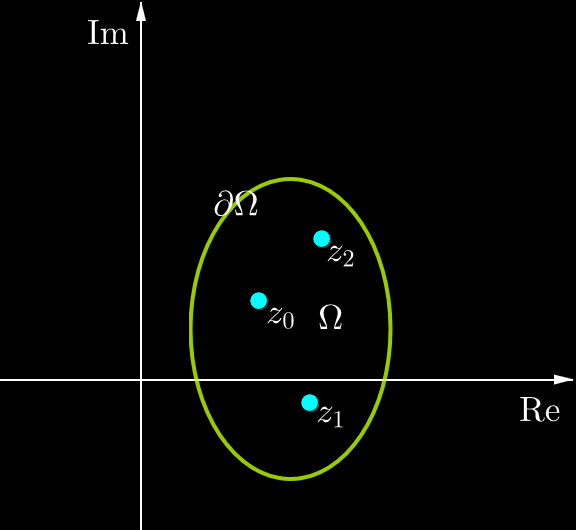
\includegraphics[scale=0.4]{4.5_residy.png}
		\caption{Tasoalue $\Omega$, jota rajoittaa käyrä $\partial\Omega$ ja jonka sisällä on kolme erikoispistettä $z_0$, $z_1$ ja $z_2$.}
	\end{figure}

	Reisdylause muuntaa siis integroinnin (jatkuva operaatio) summaukseksi (diskreetti operaatio) ja on täten erittäin voimakas tulos. Lisäksi monessa tapauksessa alueilla, joista ollaan kiinnostuttu, erikoispisteitä on vain muutama, ehkä yksi tai kaksi, jolloin summa on melko nopeasti laskettavissa.
	
	Yhtälössä (4.X) esiintyy useita lukijalle todennäköisesti uusia symboleja ja funktioita. Tämä ei estä kuitenkaan käyttämästä tulosta ja nauttimasta sen tuomista hyödyistä, mutta pintapuolinen ymmärrys yhtälön osista on erittäin hyödyllinen. Ensimmäinen mahdollisesti uusi symboli on $\oint$. Kyseessä on integraalisymboli, mutta ympyrä kertoo integroinnista jotain tärkeää: se suoritetaan suljetun käytän yli. Mikäli käyrän yli integroiminen ei ole lukijalle tuttu konsepti, on osion 5.2 tarkastelu suositeltavaa.
	
	Funktio $\res{z = z_i}f(z)$ tarkoittaa funktion $f(z)$ residyä erikoispisteessä $z_i$. Residyn määritelmä on pisteen $z_0$ ympäristössä muodostetun funktion $f(z)$ nk. Laurentin sarjakehitelmän $f(z) = \sum\limits_{n = -\infty}^{\infty}c_n(z - z_0)^{n} = \sum\limits_{n = -\infty}^{-1}a_n(z - z_0)^n + \sum\limits_{n = 0}^{\infty}b_n(z - z_0)^n$ $\frac{1}{z - z_0}$-termin etukerrointa $c_{-1} = a_{-1}$. Määritelmä saattaa kuulosta oudolta ja sen yhteyttä integrointiin on vaikea nähdä suoraan, mutta kompleksifunktioiden sarjakehitelmillä on merkittäviä yhteyksiä niiden ominaisuuksiin. Residy liittyy siis hyvin läheisesti siihen, miten funktio $f(z)$ käyttäytyy erikoispisteidensä ympäristössä ja koska myös residylauseessa erikoispisteet ovat tärkeässä asemassa, on residyn ja $f(z)$:n integraalin välinen linkki hieman ymmärrettävämpi. (Toki vieläkään ei ole perusteltu miksi erikoispisteet ovat tärkeitä funktion $f(z)$ ominaisuuksia tarkasteltaessa, sillä tähän vaadittaisiin jälleen kokonainen osio integrointiin liittymätöntä kompleksifunktioiden teoriaa.)
	
	Viimeisenä funktio $\wind(\alpha, z_i)$ tarkoittaa kiertoluku (eng. winding number), joka nimensä mukaisesti kuvaa, kuinka monta kertaa käyrä $\alpha$ kiertää pisteen $z_i$, ja mihin suuntaan. Se siis huomioi ainoastaan kulman, joka kertyy kuljettaessa $\alpha$:n yli, eli ei huomioi $\alpha$:n muotoa lainkaan. Kiertoluku jonkin pisteen $z_0$ ympäri mielivaltaisella suljetulla käyrällä $\alpha$ voidaan määrittää yhtälön (4.X) kaavalla:
	
	\begin{equation}
		\boxed{\wind(\alpha, z_0) = \frac{1}{2\pi i}\oint_{\alpha}\frac{1}{z - z_0}\odif{z}}
	\end{equation}

	Kiertoluvun määritelmä noudattaa matematiikassa tavallista kiertosuuntakonventiota, jossa vastapäivään kiertäminen on positiivinen suunta ja myötäpäivään negatiivinen. On huomattavaa, että kiertoluvun kaavassa esiintyy kerroin $\frac{1}{2\pi}$, joka vastaa jakamista kokonaisen kierroksen kulmalla. Kiertoluku ei siis mittaa kulmaa, vaan kokonaisia kierroksia! Tästä voidaan päätellä, että mikäli $\alpha$ tekee yhden kierroksen vastapäivään pisteen $z_0$ ympäri, tulee kiertoluvuksi 1 ja tämän perusteella voidaankin kirjoittaa tässä oppaassa eniten käytetty erikoistapaus residylauseesta:
	
	\begin{corollary}[\textbf{Residylauseen erikoistapaus}]
		Mikäli kaikki residylauseen (4.1) ehdot täyttyvät ja lisäksi $\alpha$ kiertää kaikki erikoispisteet $z_i$ kerran vastapäivään, yksinkertaituu integraali muotoon:
		
		\begin{equation}
			\boxed{\oint_{\alpha}f(z)\odif{z} = 2\pi i\sum_{i = 1}^{n}\res{z = z_i}f(z)}
		\end{equation}
	\end{corollary}

	Yhtälöä (4.62) voidaan soveltaa lukuisiin integraaleihin, kunhan tiedetään miten Residyjä todellisuudessä määritetään. Kuten aiemmin todettiin residy vastaa funktion $f(z)$ potenssisarjakehitelmän asteluvun $-1$ termin etukerrointa $a_{-1} = \res{z = z_0}f(z)$. Mikäli sarjakehitelmien tekeminen on lukijalle tuttua (esim. Taylorin sarjat), kykenee tämä määrittämään residyn perinteisellä tavalla. Sarjakehitelmiä osaamaton voi puolestaan hyödyntää seuraavaksi esiteltäviä tuloksia residyn määrittämiselle erilaisissa tilanteissa. Ennen tulosten esittelyä on kuitenkin ymmärrettävä vielä yksi käsite: erikoispisteen eli navan kertaluku.
	
	Funktiolla $f(z)$ on napa pisteessä $z_0$, mikäli $f(z_0)$ ei ole hyvin määritelty. Käytännössä tämä tarkoittaa, että funktiossa $f(z)$ esiintyy muotoa $\frac{1}{z - z_0}$ oleva termi, joka hajaantuu, kun $z\to z_0$. Mikäli tämä epäjatkuvuus pisteen $z_0$ ympäristössä voidaan eliminoida kertomalla $f(z)$ termillä $(z - z_0)^n$, jossa $n\in\mathbb{Z}_+$, sanotaan $z_0$:n olevan funktion $f$ $n$:nen kertaluvun napa. Esimerkiksi funktiota
	
	\begin{equation}
		f(z) = \frac{1}{z}
	\end{equation}
	
	Kerrotaessa termillä $z$:
	
	\begin{equation}
		zf(z) = z\frac{1}{z} = 1
	\end{equation}

	Saadaan napa $z = 0$ eliminoitua pois, jolloin $z = 0$ on ensimmäisen kertaluokan napa. Toinen esimerkki:
	
	\begin{equation}
		f(z) = \frac{1}{z^2 - 1}
	\end{equation}

	$z$:n arvolla $\pm i$ $f(z)$ ei ole hyvin määritelty. Jos funktiota kerrotaan termillä $(z - i)$, saadaan:
	
	\begin{align}
		(z - i)f(z) &= \frac{z - i}{z^2 - 1} \\
		\intertext{Jaetaan nimittäjä tekijöihin:}
		&= \frac{z - i}{(z - i)(z + 1)} \\
		(z - i)^2f(z) &= \frac{1}{z + i}
	\end{align}

	Havaitaan, että napa $z = i$ eliminoitui, jolloin $i$ on ensimmäisen kertaluokan napa. Vastaavasti, jos funktiota olisi kerrottu termillä $(z - (-i)) = (z + i)$, olisi napa $z = -i$ eliminoitunut, jolloin myös $-i$ on ensimmäisen kertaluokan napa. Kolmas esimerkki:
	
	\begin{equation}
		f(z) = \frac{1}{z^3 - 2z^2 + z}
	\end{equation}

	$z$:n arvoilla 0 ja 1 $f(z)$ ei ole hyvin määritelty. Nähdään suoraan, että mikäli funktiota kerrotaan $z$:lla, supistuu nimittäjän viimeinen $z$ ykköseksi, jolloin napa $z = 0$ eliminoituu eli 0 on ensimmäisen kertaluokan napa. Jos funktiota kerrotaan termillä $(z - 1)^2$, saadaan:
	
	\begin{align}
		(z - 1)^2f(z) &= \frac{(z - 1)^2}{z^3 - 2z^2 + z} \\
		\intertext{Jaetaan nimittäjä tekijöihin:}
		&= \frac{(z - 1)^2}{z(z^2 - 2z + 1)}
		&= \frac{(z - 1)^2}{z(z -  1)^2} \\
		&= \frac{1}{z}
	\end{align}

	Havaitaan, että napa $z = 1$ eliminoitui, jolloin 1 on toisen kertaluokan napa. Ei olisi siis riittänyt kertoa funktiota termillä $(z - 1)$, sillä $1$ on nimittäjän kaksoisjuuri, jolloin se esiintyy kahteen kertaan juurien tulossa. Tästä tehdäänkin tärkeä päätelmä kertalukuihin liittyen:
	
	\begin{remark}[\textbf{Navan kertaluku}]
		Sievennetyn funktion $f(z) = \frac{p(z)}{q(z)}$ mielivaltaisen navan $z_i$ kertaluku on sama kuin polynomin $q(z)$ juuriesityksessä termin $(z - z_i)^n$ eksponentti $z$, eli juuren $z_i$ moninkerta.
	\end{remark}
	
	On tärkeää, että funktio $f(z)$ on sievennetty siten, että $p$:n asteluku on pienempi kuin $q$:n, sillä jos $p$:n asteluku olisi $q$:ta suurempi, saattaisi $p$:ssä esiintyä termi, joka supistaisi $q$:n juuria pienentäen niiden moninkertaa, jolloin navan kertaluvuksi saataisiin väärä tulos.
	
	Nyt ollaan valmiita laskemaan residyjä. Yleisessä tapauksessa funktion $f(z)$ residy kertaluvun $m$ omaavan navan $z_0$ ympäristössä määritetään kaavalla:
	
	\begin{equation}
		\boxed{\res{z = z_0}f(z) = \frac{1}{(m - 1)!}\lim_{z\to z_0}\left[\odv{^{m - 1}}{x^{m - 1}}\big((z - z_0)^{m}f(z)\big)\right]}
	\end{equation}

	Kaavasta voidaan huomata seuraavat asiat: Termi $\frac{1}{(m - 1)!}$ kumoaa $m - 1$ kertaa funktiota $(z - z_0)^m$ derivoitaessa syntyvät etukertoimet. Lisäksi derivoitava lauseke $(z - z_0)^{m}f(z)$ muistuttaa suuresti napojen eliminoimiseen käytettyä taktiikkaa, jossa funktiota kerrottiin navan potenssilla. Tämä ei ole sattumaa, sillä termin $(z - z_0)^{m}$ on kuin onkin tarkoitus eliminoida $m$:nen kertaluvun napa $z_0$ funktiosta $f(z)$, jotta raja-arvo $\lim\limits_{z\to z_0}$ voidaan määrittää. Mainitsemisen arvoisia erikoistapauksia ovat ensimmäisen ($m = 1$), ja toisen kertaluvun ($m = 2$) navat, joille kaava sievenee yksinkertaisempaan muotoon:
	
	\begin{itemize}
		\item \underline{Ensimmäisen kertaluvun napa:}
		
		\begin{align}
			\res{z = z_0}f(z) &= \frac{1}{(1 - 1)!}\lim_{z\to z_0}\left[\odv{^{1 - 1}}{x^{1 - 1}}\big((z - z_0)f(z)\big)\right] \\
			&= \frac{1}{0!}\lim_{z\to z_0}\left[\odv{^0}{x^0}\big((z - z_0)f(z)\big)\right]
		\end{align}
	
		\noindent $0! = 1$ ja 0. derivaatta tarkoittaa, ettei derivaattaa lasketa lainkaan, jolloin saadaan:
		
		\begin{equation}
			\boxed{\res{z = z_0}f(z) = \lim_{z\to z_0}\Big[(z - z_0)f(z)\Big]}
		\end{equation}
	
		\item \underline{Toisen kertaluvun napa:}
		
		\begin{align}
			\res{z = z_0}f(z) &= \frac{1}{(2 - 1)!}\lim_{z\to z_0}\left[\odv{^{2 - 1}}{x^{2 - 1}}\big((z - z_0)^2f(z)\big)\right] \\
			&= \frac{1}{1!}\lim_{z\to z_0}\left[\odv{}{x}\big((z - z_0)^2f(z)\big)\right]
		\end{align}
	
		\noindent $1! = 1$, jolloin saadaan:
		
		\begin{equation}
			\boxed{\res{z = z_0}f(z) = \lim_{z\to z_0}\left[\odv{}{x}\big((z - z_0)^2f(z)\big)\right]}
		\end{equation}
	\end{itemize}

	
	\subsubsection{Rationaalifunktkioiden epäoleelliset integraalit}
	
	\begin{figure}[h!]
		\centering
		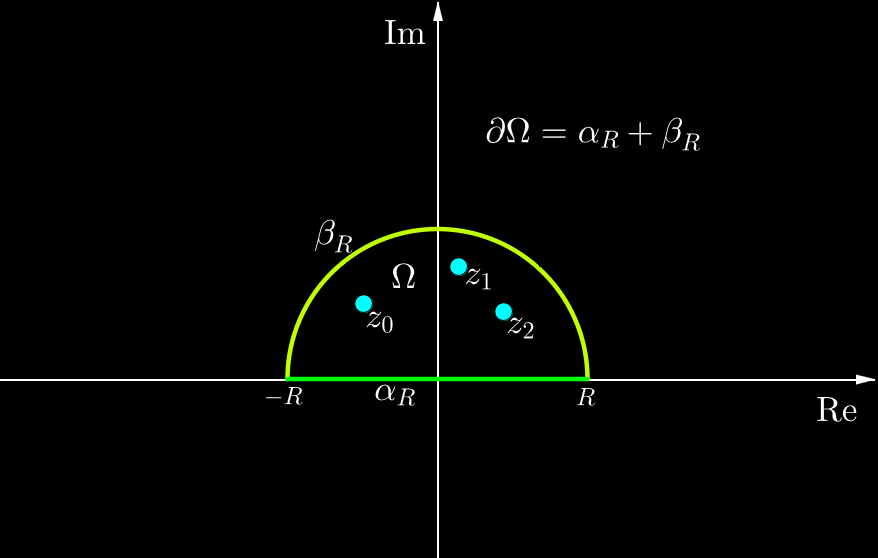
\includegraphics[scale=0.3]{4.5_ylakeha.png}
		\caption{Epäoleellisten integraalien määrittämisessä käytetty ylemmässä puolitasossa sijaitseva integroimisreitti $\partial\Omega$.}
	\end{figure}
	
	Ensimmäinen integraalityyppi, jonka määrittämisessä residylauseestä on hyöytyä, ovat rationaalifunktioiden $r(x) = \frac{p(x)}{q(x)}$ epäoleelliset integraalit:
	
	\begin{equation}
		I = \int_{-\infty}^{\infty}r(x)\odif{x} = \int_{-\infty}^{\infty}\frac{p(x)}{q(x)}\odif{x}
	\end{equation}

	Residylausetta voidaan käyttää suoraan tällaisiin epäoleellisiin integraaleihin, kunhan seuraavat ehdot toteutuvat:
		
	\begin{itemize}
		\item $p$:n asteluku $n$ on vähintään $q$:n astelukua $m$ kaksi pienempi: $m \geq n + 2$
		\item $q$:lla ei ole reaalisia nollakohtia
	\end{itemize}
	
	Nyt integraali $I$ voidaan määrittää laajentamalla integroimispolku reaaliakselilta kompleksitasoon ympäröiden esimerkiksi kaikki $q$:n ylemmässä puolitasossa sijaitsevat navat puoliympyrän kaarella vastapäivään (ks. kuva 4.2), jolloin reunakäyrän $\partial\Omega$ yli integroiminen tuottaa residylauseen perusteella:
	 
	\begin{align}
		\oint_{\partial\Omega}r(z)\odif{z} &= 2\pi i\sum_{i = 1}^{n}\res{z = z_i}r(z) \\
		\intertext{Yhtälön vasemman puolen integraali ei vielä ole haluttu integraali $I$, mutta tämä muuttuu kun polkuintegraali $\partial\Omega$:n yli kirjoitetaan tuloksen (3.7) nojalla osapolkujen  $\alpha_R$ ja $\beta_R$ integraalien summana:}
		\int_{\alpha_R}r(z)\odif{z} + \int_{\beta_R}r(z)\odif{z} &= 2\pi i\sum_{i = 1}^{n}\res{z = z_i}r(z) \\
		\intertext{Polku $\alpha_R$ on yksinkertaisesti reaaliakselin lukuväli $[-R, R]$, jolloin integrointi voidaan suorittaa tavallisena integraalina $x$:n suhteen:}
		\int_{-R}^{R}r(x)\odif{x} + \int_{\beta_R}r(z)\odif{z} &= 2\pi i\sum_{i = 1}^{n}\res{z = z_i}r(z) \\
		\intertext{Otetaan raja-arvo $R\to\infty$. Koska käyrä $\partial\Omega$ sisältää kaikki $q$:n yläpuolitason navat tarpeeksi suurella $R$:n arvolla, ei yhtälön oikea puoli muutu lainkaan:}
		\lim_{R\to\infty}\int_{-R}^{R}r(x)\odif{x} + \lim_{R\to\infty}\int_{\beta_R}r(z)\odif{z} &= 2\pi i\sum_{i = 1}^{n}\res{z = z_i}r(z) \\
		\intertext{Ensimmäinen integraali tulee integraalin $I$ muotoiseksi. Ratkaistaan tämän suhteen:}
		\int_{-\infty}^{\infty}r(x)\odif{x} &= 2\pi i\sum_{i = 1}^{n}\res{z = z_i}r(z) - \lim_{R\to\infty}\int_{\beta_R}r(z)\odif{z}
	\end{align}

	Nyt integraali $I$ voidaan määrittää, kunhan tiedetään, mitä toisen integraalin arvoksi tulee. Koska $p$ ja $q$ ovat polynomeja, ohjaa niiden käytöstä suurilla $|z|$:n arvoilla niiden korkeimman asteluvun termi, jolloin voidaan aina löytää vakiot $C_1$ ja $C_2$, joille $|p(z)| \leq C_1|z|^n$ ja $|q(z)| \geq C_2|z|^m$. Hyödyntäen näitä lausekkeita, voidaan integraalille puolikaaren yli löytää yläraja. Sijoittamalla termit $C_1|z|^n$ ja $C_2|z|^m$ $p$:n ja $q$:n tilalle, saadaan epäyhtälö:
	
	\begin{align}
		\lim_{R\to\infty}\int_{\beta_R}\left|\frac{p(z)}{q(z)}\right|\odif{z} &\leq \lim_{R\to\infty}\int_{\beta_R}\frac{C_1|z|^n}{C_2|z|^m}\odif{z} \\
		\intertext{Epäyhtälö pätee, koska oikean puolen jaettava $C_1|z|^n$ on suurempi vasemman puolen jaettava $|p(z)|$ ja oikean puolen jakaja $C_2|z|^m$ on pienempi kuin vasemman puolen jakaja $|q(z)|$ tuottaen oikealle puolelle suuremman luvun. Merkitään suhdetta $\frac{C_1}{C_2} = C$. Koska vaatimuksena oli, että $m \geq n + 2$, valitaan kaikkein lähimpänä rajaa oleva tapaus $m = n + 2$, sillä mikäli tällä tavalla saadaan jokin tulos, pätee se myös kaikille $m > n + 2$. Saadaan:}
		\left|\lim_{R\to\infty}\int_{\beta_R}\frac{p(z)}{q(z)}\odif{z}\right| &\leq \lim_{R\to\infty}\int_{\beta_R}\frac{C}{|z|^2}\odif{z} \\
		\intertext{Itseisarvo $|z|$ vastaa kompleksiluvun sädettä, joka on $R$-säteisen puoliympyrän yli integroitaessa $R$:}
		\left|\lim_{R\to\infty}\int_{\beta_R}\frac{p(z)}{q(z)}\odif{z}\right| &\leq \lim_{R\to\infty}\int_{\beta_R}\frac{C}{R^2}\odif{z} \\
		\intertext{Säde $R$ on integroinnin suhteen vakio, jolloin se voidaan ottaa integraalin ulkopuolelle:}
		\left|\lim_{R\to\infty}\int_{\beta_R}\frac{p(z)}{q(z)}\odif{z}\right| &\leq \lim_{R\to\infty}\frac{C}{R^2}\int_{\beta_R}\odif{z} \\
		\intertext{Integrointi $R$-säteisen puoliympyrän yli tuottaa puoliympyrän kaaren pituuden $\pi R$:}
		\left|\lim_{R\to\infty}\int_{\beta_R}\frac{p(z)}{q(z)}\odif{z}\right| &\leq \lim_{R\to\infty}\frac{C}{R^2}\pi R \\
		\left|\lim_{R\to\infty}\int_{\beta_R}\frac{p(z)}{q(z)}\odif{z}\right| &\leq \lim_{R\to\infty}\frac{\pi C}{R} \\
		\intertext{Oikean puolen raja-arvo menee nollaan, jolloin saadaan:}
		\left|\lim_{R\to\infty}\int_{\beta_R}\frac{p(z)}{q(z)}\odif{z}\right| &\leq 0 \\
		\intertext{Mikäli kaari-integraalin itseisarvo on korkeintaan nolla, voi sillä olla vain yksi arvo, eli nolla, jolloin voidaan todeta:}
		\lim_{R\to\infty}\int_{\beta_R}\frac{p(z)}{q(z)}\odif{z} &= 0
	\end{align}

	On siis osoitettu, että yhtälön (4.X) kaari-integraali menee nollaan, jolloin lopulliseksi tulokseksi epäoleelliselle integraalille saadaan:
	
	\begin{equation}
		\boxed{\int_{-\infty}^{\infty}r(x)\odif{x} = 2\pi i\sum_{i = 1}^{n}\res{z = z_i}r(z)}
	\end{equation}

	Tulosta voidaan siis käyttää sillä ehdolla, että $q$:n asteluku on vähintään kahdella suurempi $p$:n astelukua ja $q$:lla ei ole napoja reaaliakselilla. Ensimmäisen ehdon perustelu on nyt jälkikäteen helpompaa, sillä mikäli $q$:n asteluku olisi esimerkiksi vain yhden $p$:n astelukua suurempi, olisi kaari-integraalissa ollut integroitavana funktio $\frac{1}{R}$, jolloin olisi pätenyt:
	
	\begin{align}
		\lim_{R\to\infty}\int_{\beta_R}\frac{C}{R}\odif{z} &= \lim_{R\to\infty}\frac{C}{R}\int_{\beta_R}\odif{z} \\
		&= \lim_{R\to\infty}\frac{C}{R}\pi R \\
		&= \lim_{R\to\infty}\pi C \\
		&= \pi C
	\end{align}

	Kaari-integraali ei olisi enää mennyt nollaan ja se olisi pitänyt laskea erikseen. Vieläpä jos $p$:n asteluku olisi yhtä suuri kuin $q$:n asteluku, pätisi:
	
	\begin{align}
		\lim_{R\to\infty}\int_{\beta_R}C\odif{z} &= \lim_{R\to\infty}C\int_{\beta_R}\odif{z} \\
		&= \lim_{R\to\infty}C\pi R \\
		&= \infty
	\end{align}

	Kaari-integraali olisi siis hajaantununut, jolloin myös alkuperäinen integraali olisi hajaantunut. Tästä syystä ehto $m \geq n + 2$ on hyvin perusteltu, ja tulemme vastaisuudessa perustelemaan integraalien katoamista mm. vetomalla yllä johdettuun tulokseen.


	\begin{figure}[h!]
		\centering
		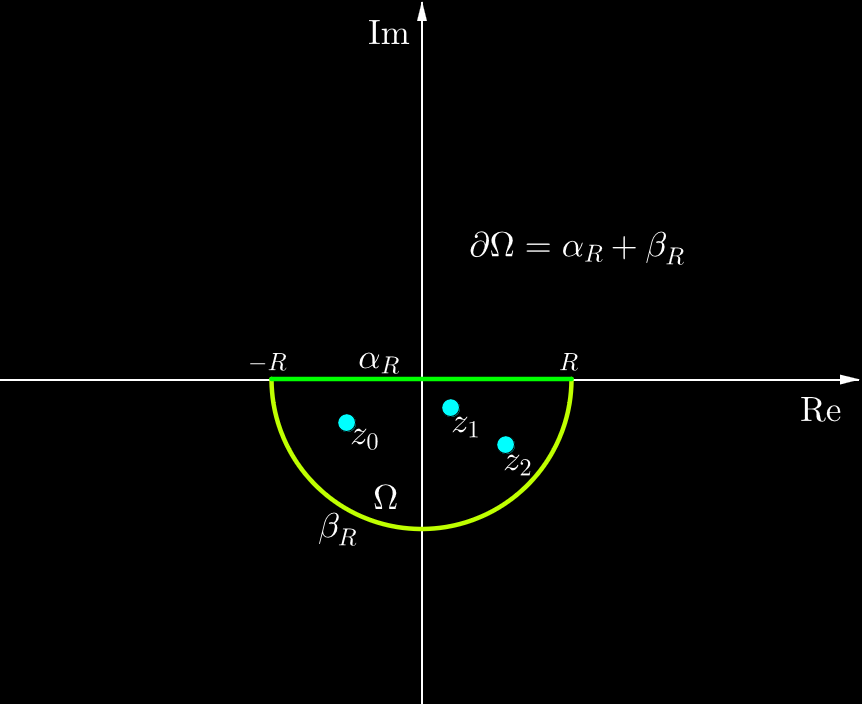
\includegraphics[scale=0.3]{4.5_alakeha.png}
		\caption{Epäoleellisten integraalien määrittämisessä käytetty alemmassa puolitasossa sijaitseva integroimisreitti $\partial\Omega$.}
	\end{figure}

	\subsubsection{Pääarvointegraalit}
	
	
	\begin{figure}[h!]
		\centering
		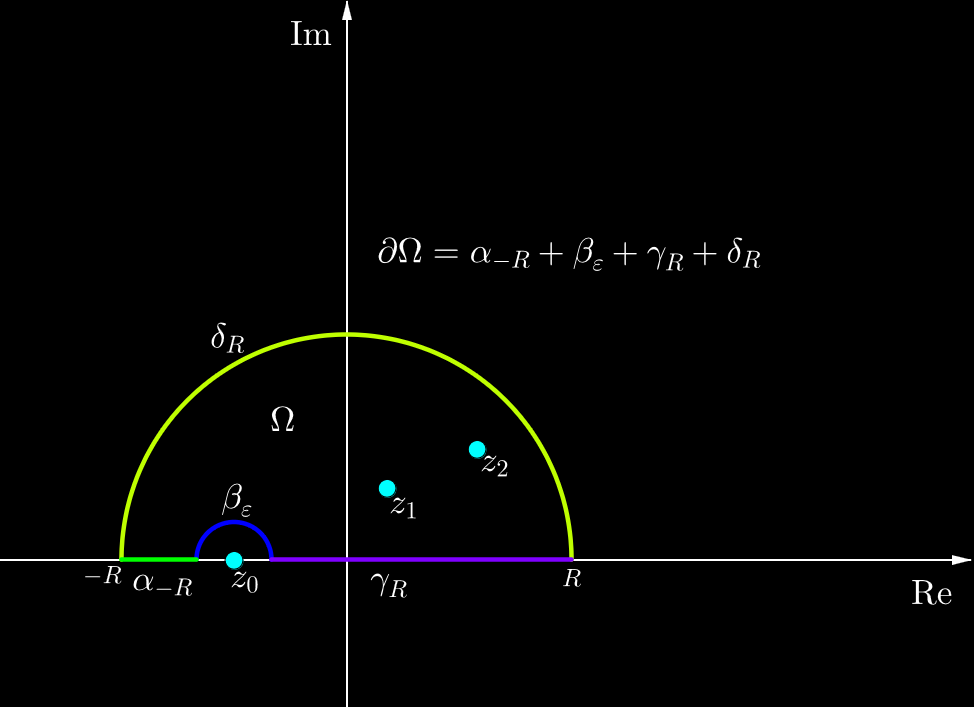
\includegraphics[scale=0.3]{4.5_paa-arvo.png}
		\caption{Epäoleellisten integraalien määrittämisessä käytetty ylemmässä puolitasossa sijaitseva integroimisreitti $\partial\Omega$, kun integrandilla on napa $z_0$ reaaliakselilla.}
	\end{figure}

	\subsubsection{Integrointi leikkauskäyrän yli}
	
	\begin{figure}[h!]
		\centering
		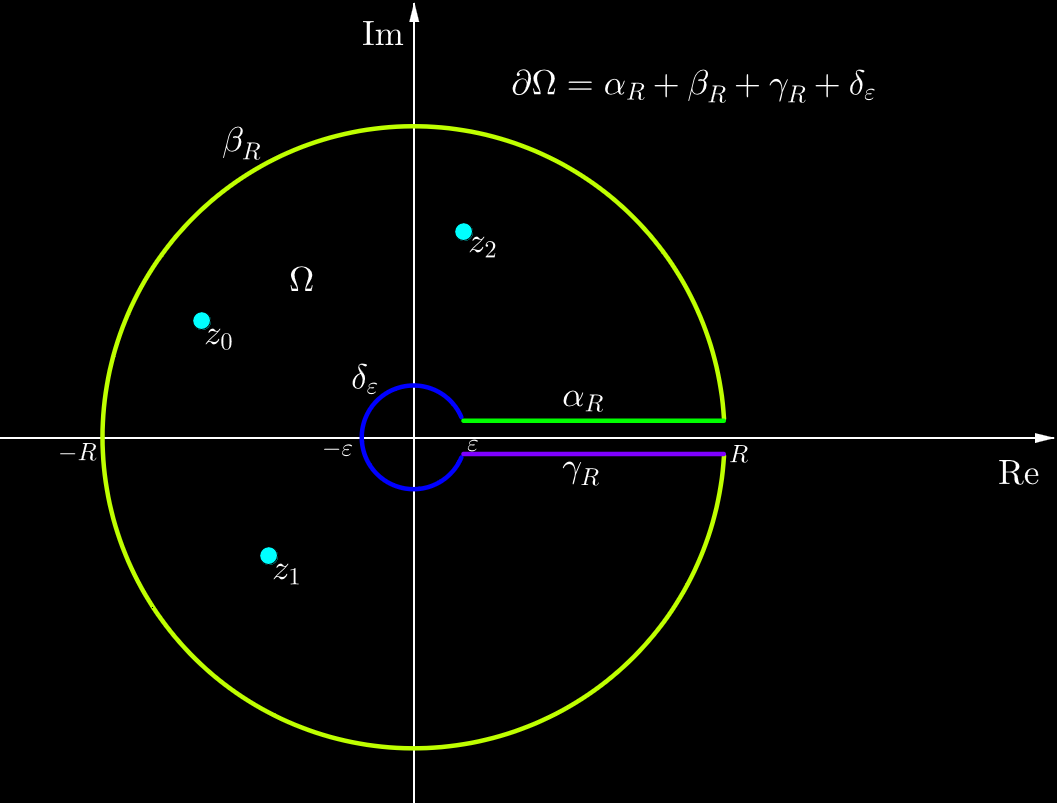
\includegraphics[scale=0.3]{4.5_avaimenreika.png}
		\caption{Erityisesti juuri- ja logaritmifunktioiden integroimisessa käytetty avaimenreikää muistuttava polku $\partial\Omega$.}
	\end{figure}

	\begin{figure}[h!]
		\centering
		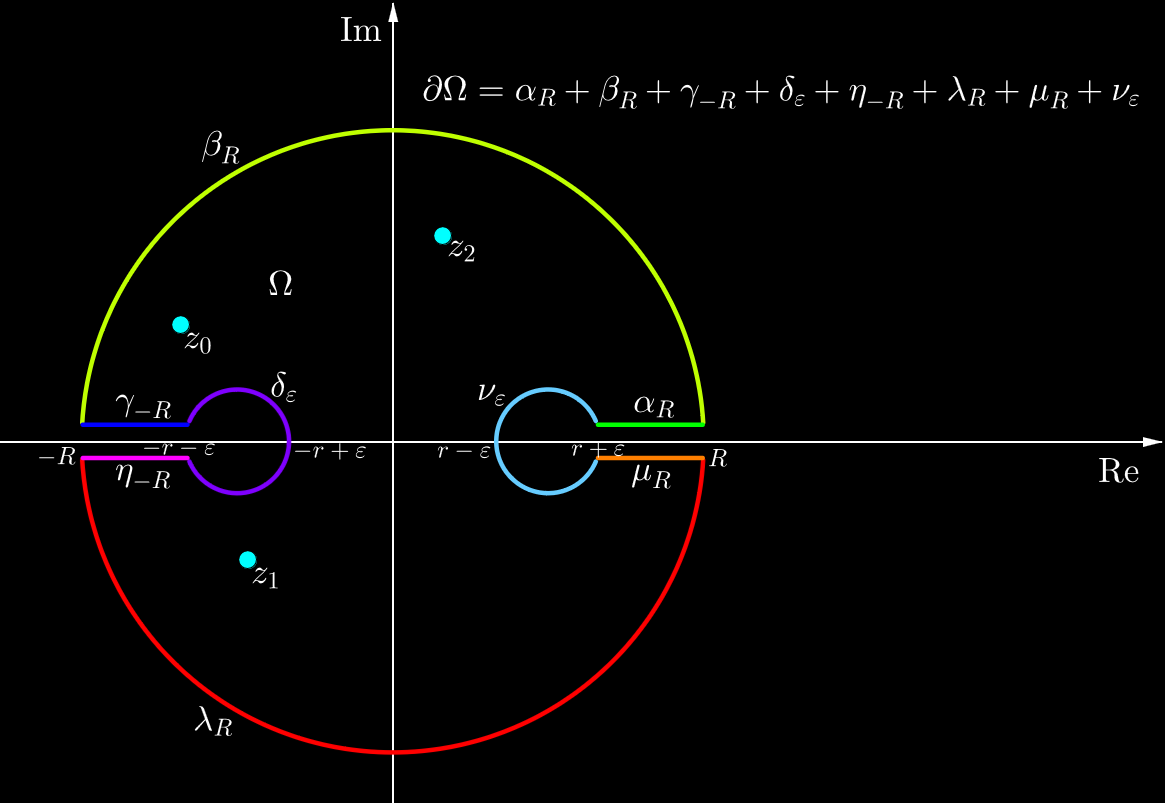
\includegraphics[scale=0.3]{4.5_kaksoisavainreika.png}
		\caption{Joissakin leikkauskäyräintegraaleissa esiintyvä ''kaksoisavaimenreikä'' $\partial\Omega$.}
	\end{figure}

	\begin{figure}[h!]
		\centering
		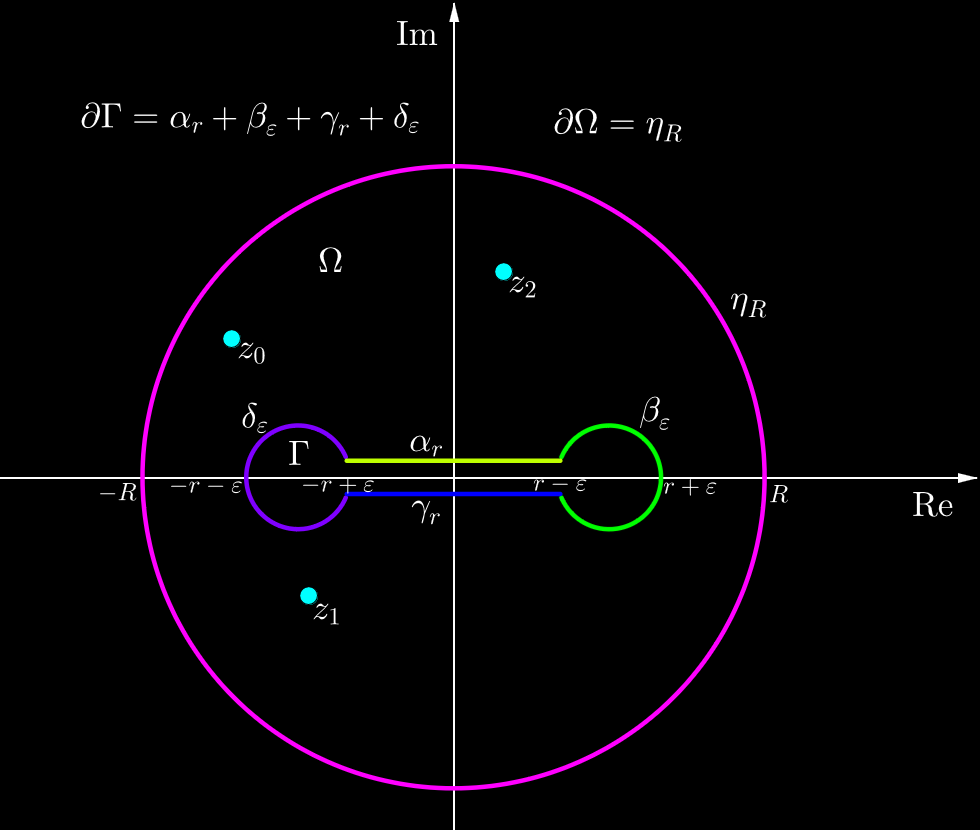
\includegraphics[scale=0.3]{4.5_koiranluu.png}
		\caption{Joissakin leikkauskäyräintegraaleissa esiintyvä ''koiranluu'' $\partial\Omega$.}
	\end{figure}

	\subsection{Integrointi sarjakehitelmällä}

	\subsection{Glasserin yleislause}
	
	
\end{document}
